%\vspace{-0.1cm}
\section{Experiments}\label{sec:experiments}
%\vspace{-0.1cm}
% In this section, we present our empirical evaluations of \opacex. 
We evaluate \opacex on the Pendulum-v1 and MountainCar environment from the OpenAI gym benchmark suite~\citep{brockman2016openai}, on the Reacher, Swimmer, and Cheetah from the deep mind control suite~\citep{tassa2018deepmind}, and a high-dimensional simulated robotic manipulation task introduced by~\citet{li2020towards}. See \Cref{sec:experiment_details} for more details on the experimental setup. 
%\vspace{-0.1cm}
\paragraph{Baselines}
\looseness=-1
We implement four baselines for comparisons. To show the benefit of our intrinsic reward, we compare \opacex to (\emph{1}) a random exploration policy (\textsc{Random}) which randomly samples actions from the action space. As we discuss in \Cref{sec:opacex} our choice of objective in \Cref{eq:exploration_op} is in essence similar to the one proposed by~\cite{pathak2019self} and \cite{sekar2020planning}. Therefore, in our experiments, we compare the optimistic planner with other planning approaches.
Moreover, most work on active exploration either uses the mean planner or does not specify the planner (c.f., \Cref{sec:related_works}). We use the most common planners: (\emph{2}) mean (\textsc{Mean-AE}), and (\emph{3}) trajectory sampling (TS-1) scheme proposed in \cite{chua2018pets} (\textsc{PETS-AE}) as our baselines.
%Furthermore, we also compare our optimistic planner with a (\emph{ii}) mean planner (\textsc{Mean-AE}) and (\emph{iii}) trajectory sampling (TS-1) scheme proposed in \cite{chua2018pets} (\textsc{PETS-AE}). 
The mean planner simply uses the mean estimate $\vmu_n$  of the well-calibrated model. 
This is also used in \cite{active_learning_gp}.
%Most work on active exploration either uses the mean planner or does not specify the planner (c.f.,\Cref{sec:related_works}).
%Therefore,  we use the most common planners: mean, and trajectory sampling as our baselines.
Finally, we compare \opacex to (\emph{4}) H-UCRL~\citep{curi2020efficient}, a single-task model-based RL algorithm.
We investigate the following three aspects: (\emph{i}) {\em how fast does active exploration reduce model's epistemic uncertainty $\vsigma_n$ with increasing $n$}, (\emph{ii}) {\em can we solve downstream tasks with \opacex}, and (\emph{iii}) {\em does \opacex scale to high-dimensional and challenging object manipulation tasks}? For our experiments, we use GPs and probabilistic ensembles (PE,~\cite{lakshminarayanan2017simple}) for modeling the dynamics. For the planning, we either the soft actor-critic (SAC, \cite{sac}) policy optimizer, which takes simulated trajectories from our learned model to train a policy, or MPC with the iCEM optimizer~\citep{iCem}.
\begin{figure}[th]
    \centering
    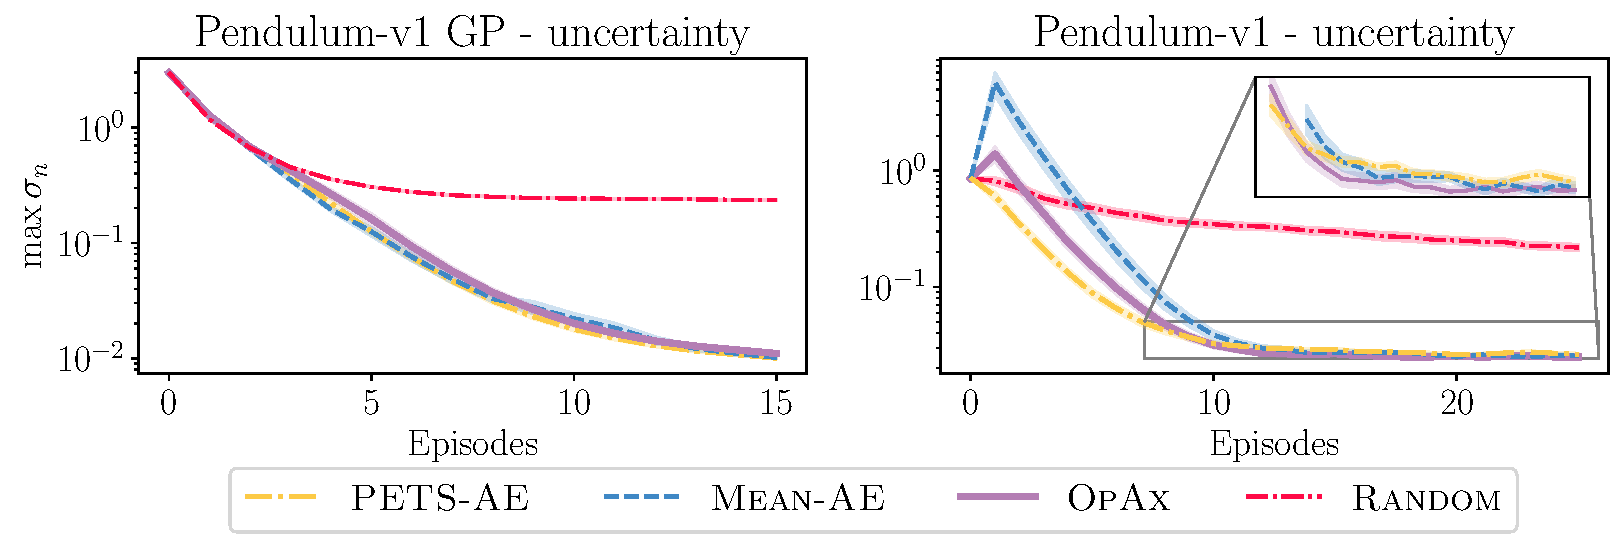
\includegraphics[width=0.75\textwidth]{figures/uncertainty_plotvalidation_eps_std_max.pdf}
    \caption{\looseness -1 Reduction in maximum epistemic uncertainty in \emph{reachable} state-action space for the Pendulum-v1 environment over 10 different random seeds. We evaluate \opacex with both GPs and PE and plot the mean performance with two standard error confidence intervals. For both, active exploration reduces epistemic uncertainty faster compared to random exploration. All active exploration baselines perform well for the GP case, whereas for the PE case \opacex gives slightly lower uncertainties.}
    \label{fig:epistemic_uncertainty_figure}
    %\vspace{-0.5cm}
\end{figure}
\begin{figure}[ht]
%\vspace{-0.2cm}
    \centering
    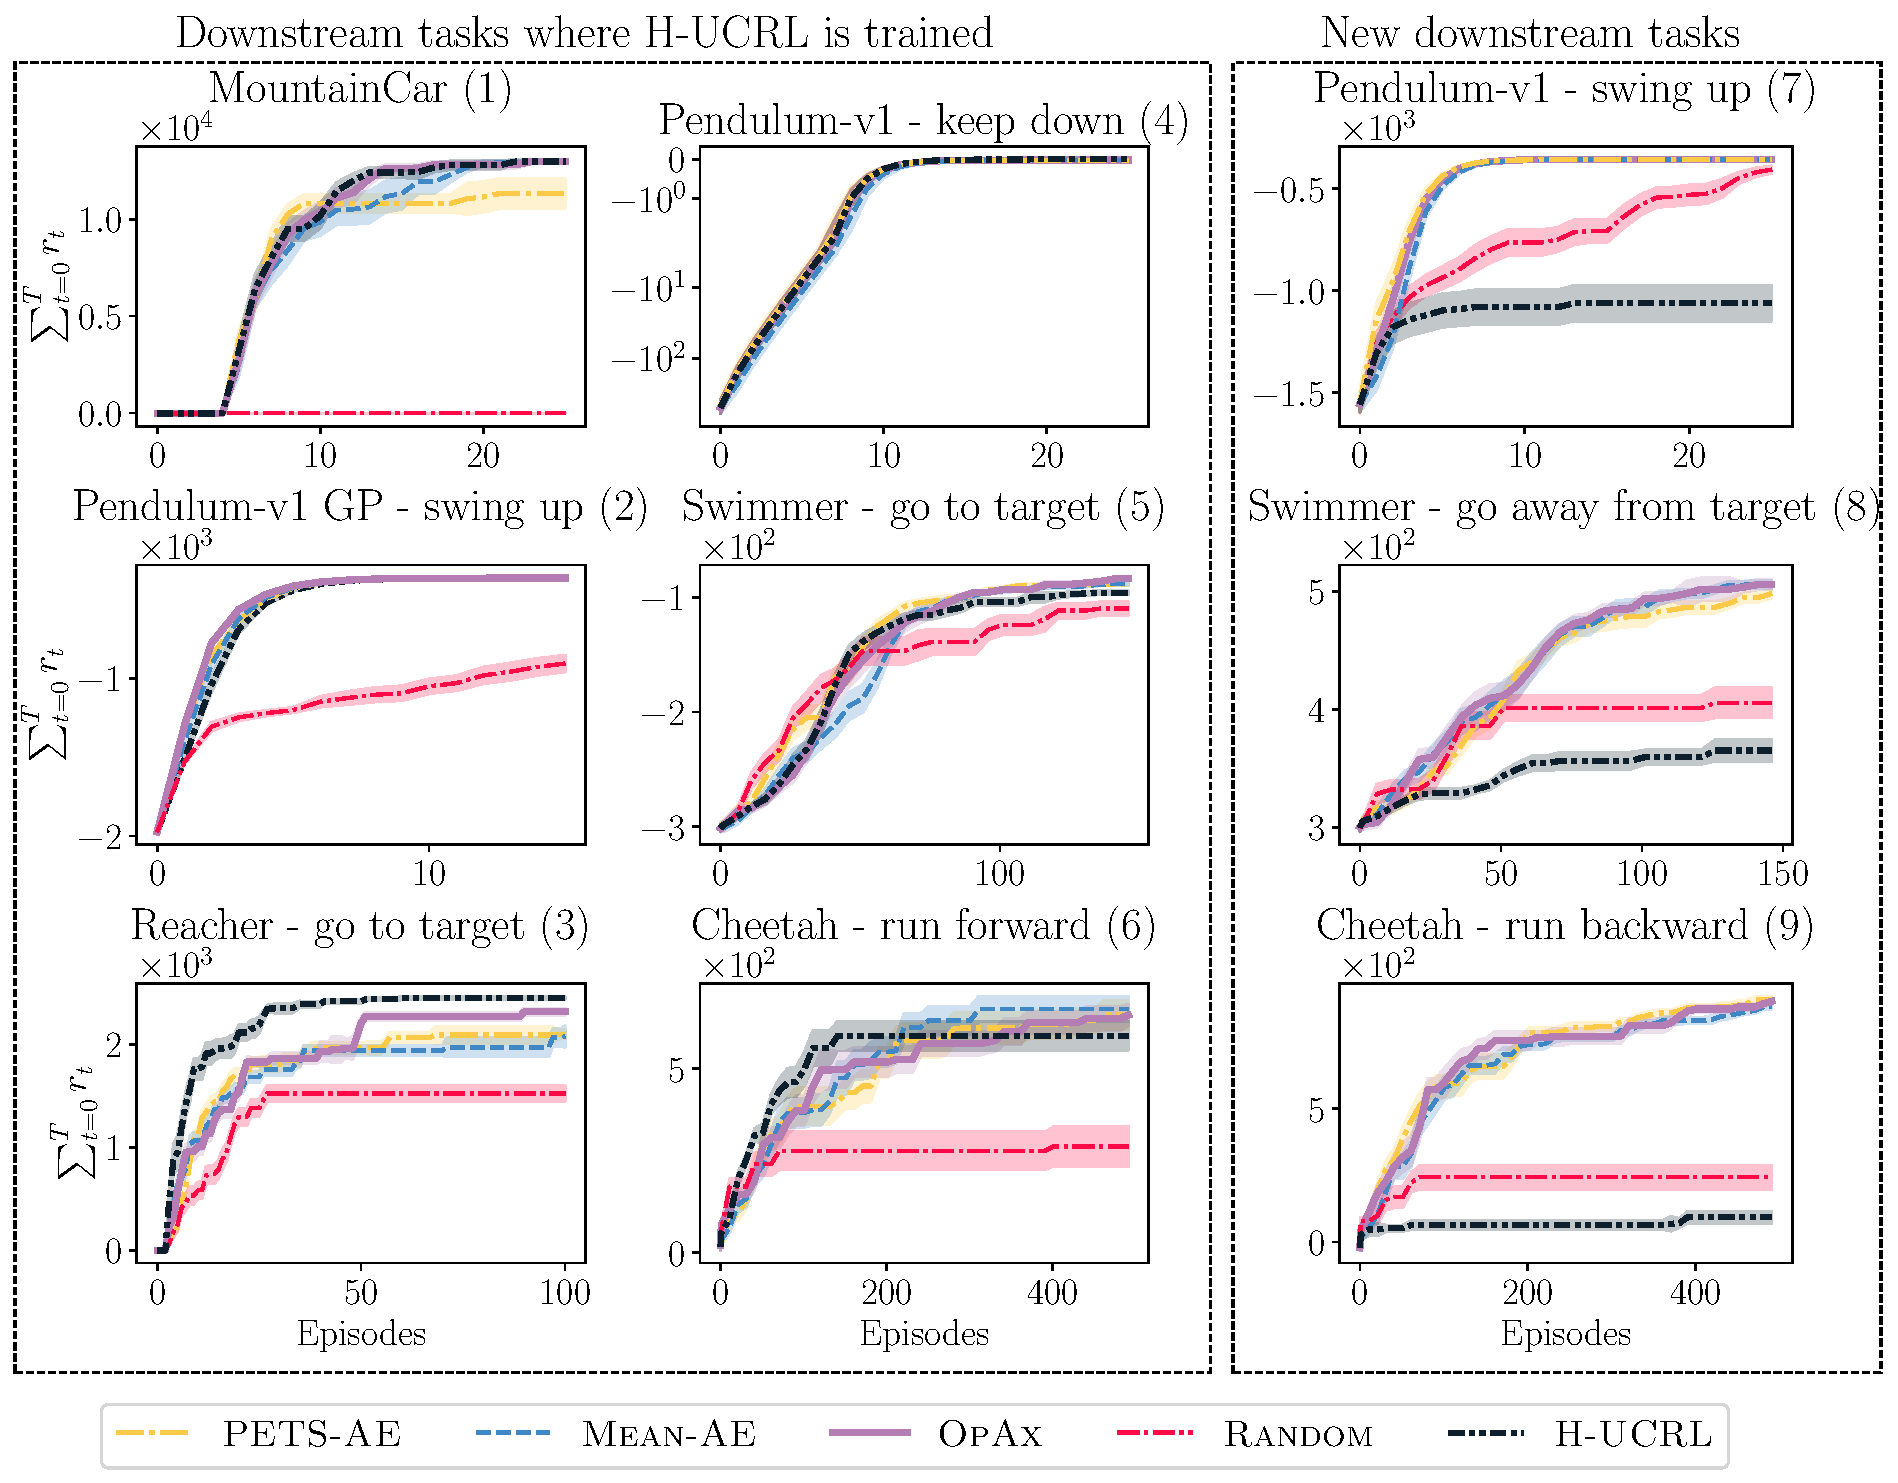
\includegraphics[width=1\textwidth]{figures/results_plot_with_hucrlreward_task_1.pdf}
    \caption{\capt{\looseness-1 We evaluate the downstream performance of our agents over 10 different random seeds and plot the mean performance with two standard error confidence intervals.
    For all the environments we use PE as models, except plot (1), for which we use a GP model (see plot (2) in the figure above). For tasks (1)-(6), we also train \textsc{H-UCRL}, a model-based RL algorithm. Tasks (7)-(9) are new/unseen for \textsc{H-UCRL}. From the Figure, we conclude that (\emph{i}) compared to other active exploration baselines, \opacex constantly performs well and is on par with \textsc{H-UCRL}, and (\emph{ii}) on the new/unseen tasks the active exploration baselines and \opacex outperform \textsc{H-UCRL} by a large margin.
    }}
%\vspace{-0.3cm}
    \label{fig:results_figure}
\end{figure}
%\vspace{-0.1cm}

\paragraph{How fast does active exploration reduce the epistemic uncertainty?}
For this experiment, we consider the Pendulum-v1 environment. We sample transitions at random from the pendulum's \emph{reachable} state-action space and evaluate our model's epistemic uncertainty for varying episodes and baselines. We model the dynamics with both GPs and PE. We depict the result
in \Cref{fig:epistemic_uncertainty_figure}. We conclude that the \textsc{Random} agent is slower in reducing the uncertainty compared to other active exploration methods for both GP and PE models. In particular, from the experiment, we empirically validate \Cref{thm:gp_theorem} for the GP case and also conclude that empirically even when using PE models, we find convergence of epistemic uncertainty. Moreover, we notice for the PE case 
that \opacex reaches smaller uncertainties slightly faster than \textsc{Mean-AE} and \textsc{PETS-AE}. We believe this is due to the additional exploration induced by the optimistic planner. 


%\vspace{-0.1cm}
\paragraph{Can the model learnt through \opacex solve downstream tasks?}
\looseness=-1
We use \opacex and other active exploration baselines to actively learn a dynamics model and then evaluate the learned model on downstream tasks. We consider several tasks, (\emph{i}) Pendulum-v1 swing up, (\emph{ii})  Pendulum-v1 keep down (keep the pendulum at the stable equilibria), (\emph{iii}) MountainCar, (\emph{iv}) Reacher - go to target, (\emph{v}) Swimmer - go to target, 
(\emph{vi}) Swimmer - go away from target (quickly go away from the target position), 
(\emph{vii}) Cheetah - run forward, (\emph{viii}) Cheetah - run backward. For all tasks, we consider PEs, except for (\emph{i}) where we also use GPs. Furthermore,
for the MountainCar and Reacher, we give a reward once the goal is reached. Since this requires long-term planning, we use a SAC policy for these tasks. We use MPC with iCEM for the remaining tasks. We also train \textsc{H-UCRL} on tasks (\emph{i}) with GPs, and (\emph{ii}), (\emph{iii}), (\emph{iv}), (\emph{v}), (\emph{vii}) with PEs. We report the best performance across all episodes. 
%(\emph{i}) MountainCar, (\emph{ii}) Reacher - go to target, where we ask the Reacher's end-effector to reach a desired goal, (\emph{iii}) Swimmer - go to target, here the goal is for the Swimmer to move towards a target, and (\emph{iv}) Cheetah - run forward, where we give positive reward for the Cheetah's forward velocity. For the MountainCar and Reacher tasks, we only give a positive reward if the goal is reached. Since this requires long-term planning, we use a SAC policy for these tasks. We use MPC with iCEM for the remaining tasks. 

To make a fair comparison, we use the following evaluation procedure; first, we perform active exploration for each episode on the environment, and then after every few episodes we use the mean estimate $\vmu_n$ to evaluate our learned model on the downstream tasks. 

\looseness=-1
\Cref{fig:results_figure} shows that all active exploration variants perform considerably better than the \textsc{Random} agent. In particular, for the MountainCar, the \textsc{Random} agent is not able to solve the task. Moreover, \textsc{PETS-AE} performs slightly worse than the other exploration baselines in this environment.
In general, we notice that \opacex always performs well and is able to achieve \textsc{H-UCRL}'s performance on all the tasks for which \textsc{H-UCRL} is trained. 
However, on tasks that are new/unseen for \textsc{H-UCRL}, active exploration algorithms outperform \textsc{H-UCRL}. 
From this experiment, we conclude two things 
(\emph{1}) apart from providing theoretical guarantees, the model learned through \opacex 
also performs well in downstream tasks, and (\emph{2}) active exploration agents generalize well to downstream tasks, whereas \textsc{H-UCRL} performs considerably worse on new/unseen tasks.
We believe this is because, unlike active exploration agents, task-specific model-based RL agents only explore the regions of the state-action space that are relevant to the task at hand.

%\vspace{-0.1cm}
\paragraph{Does \opacex scale to high-dimensional and challenging object manipulation tasks?}
\begin{wrapfigure}[13]{r}{0.2\textwidth}
%\vspace{-1.8cm}
    \label{fig:fpp_pic}
    \centering
    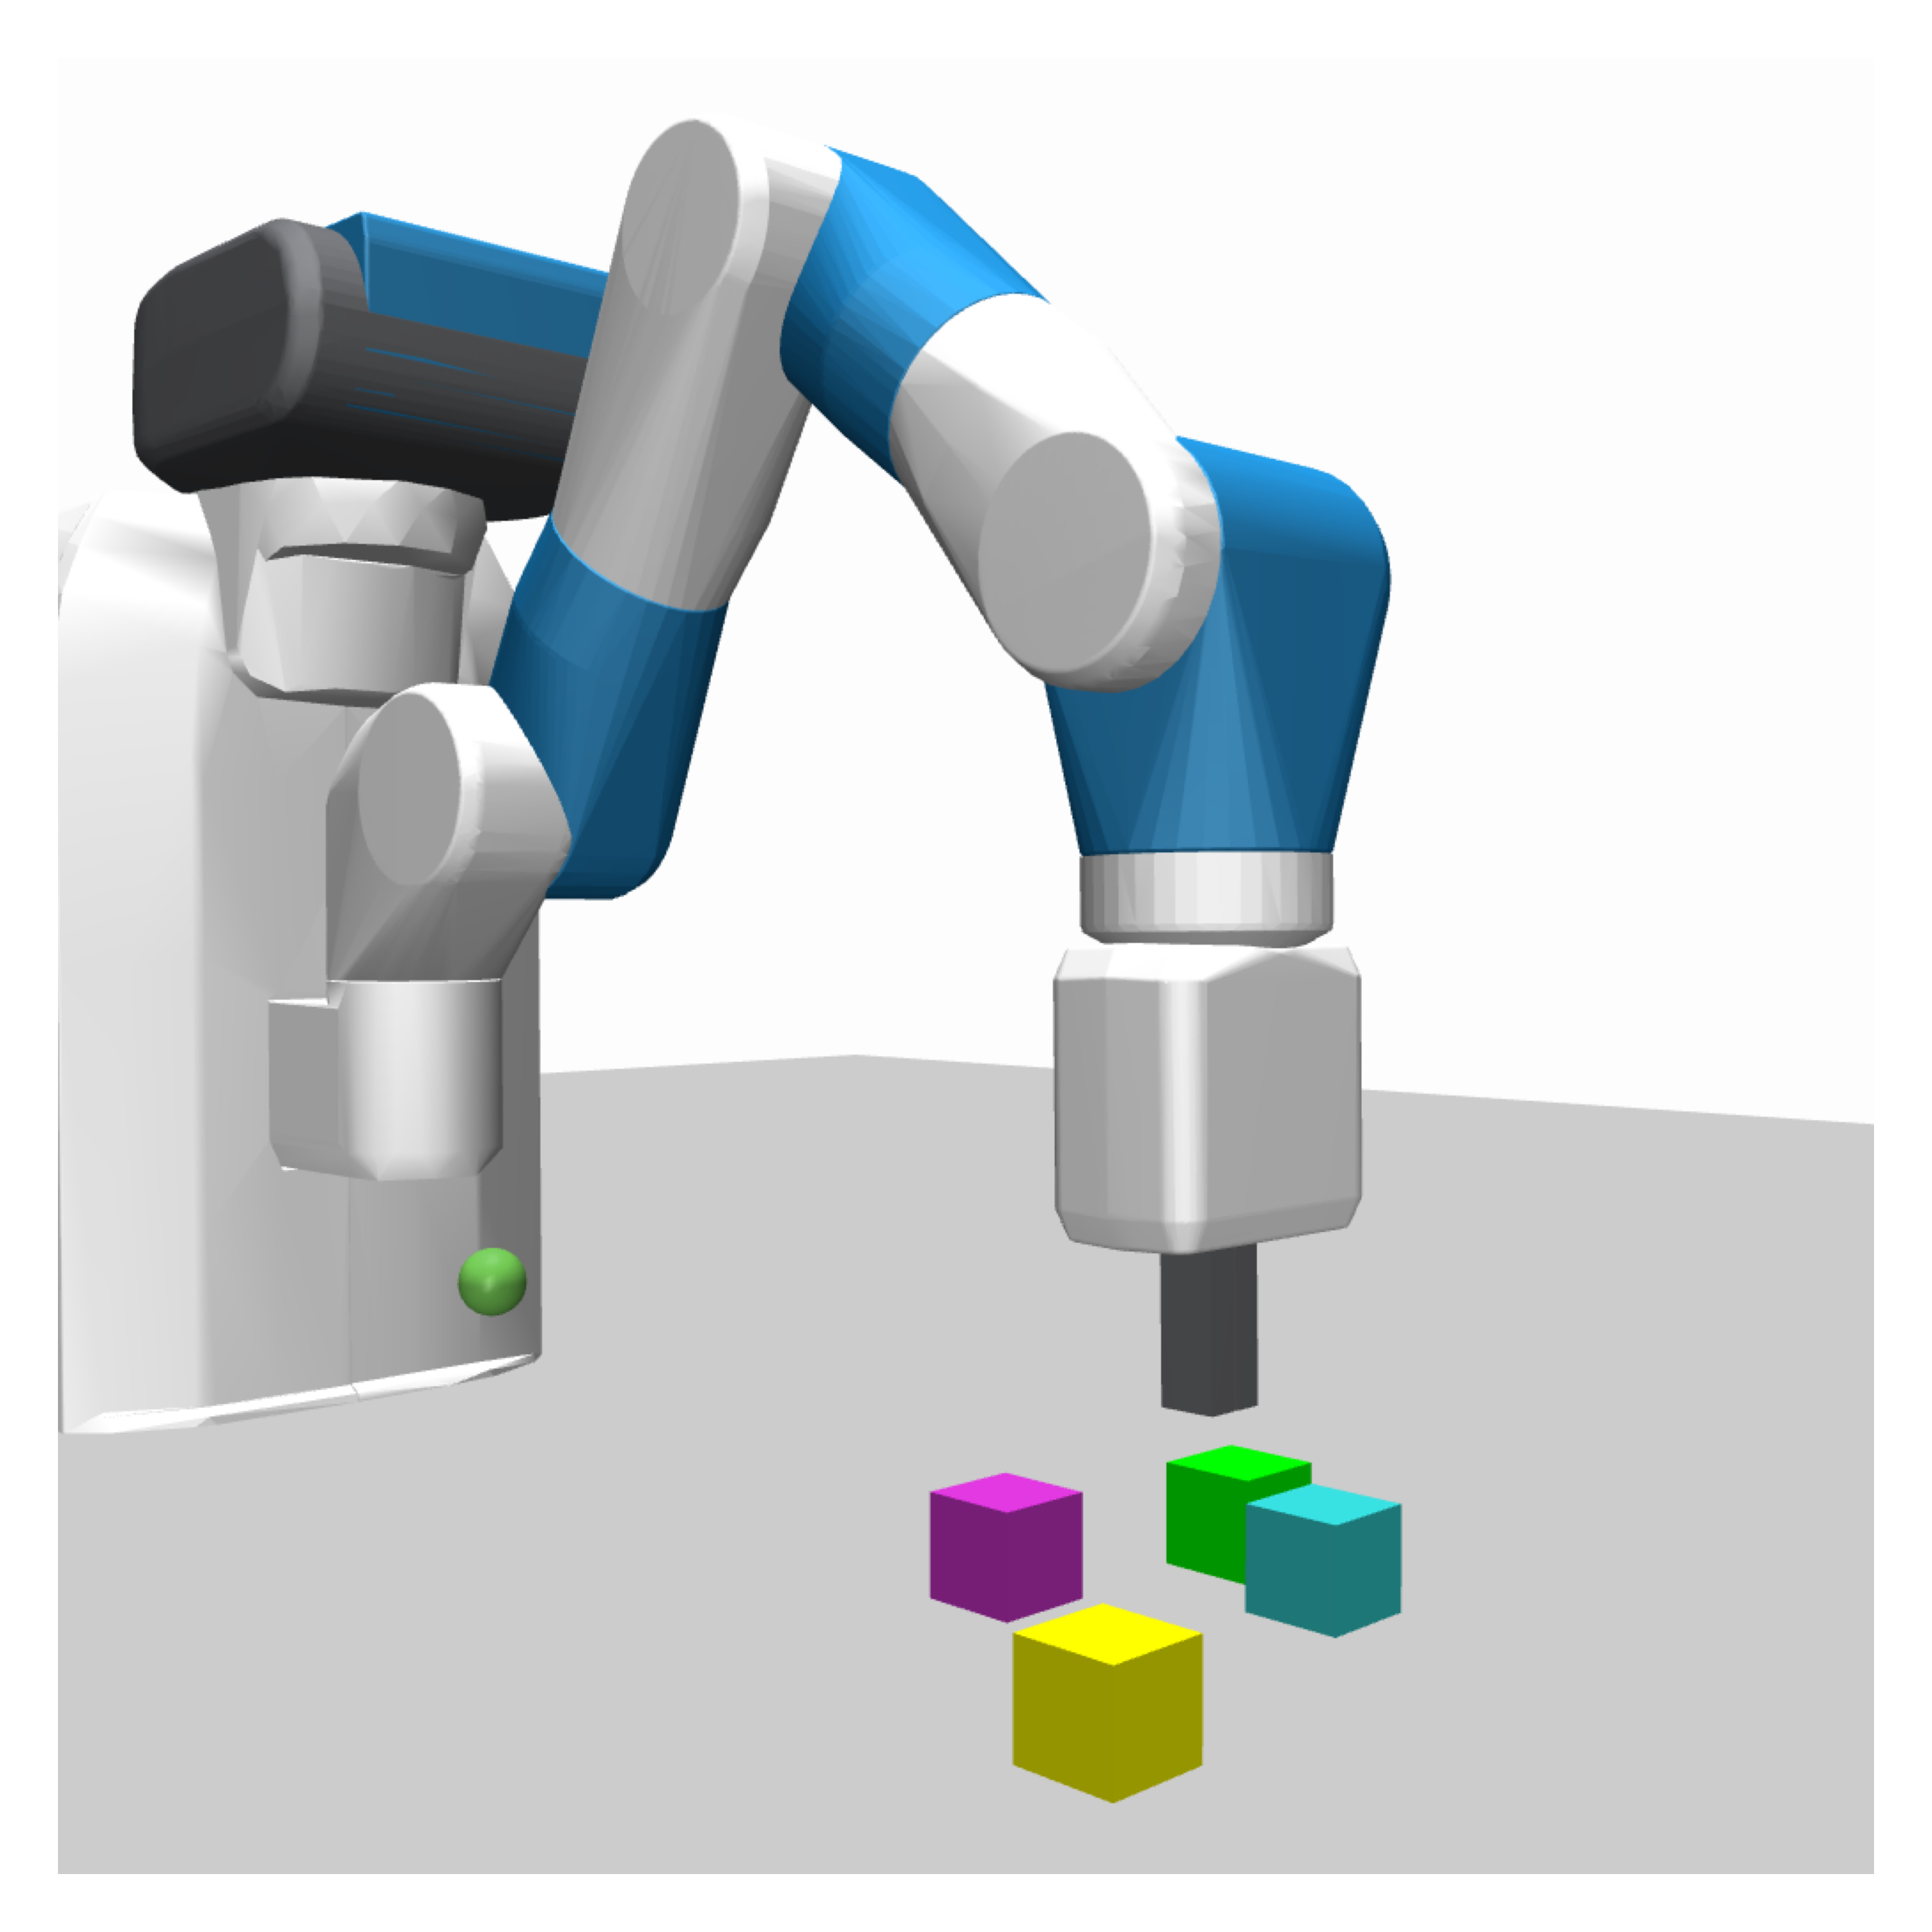
\includegraphics[width=\linewidth]{figures/fpp_construction/env_4obj.png}%\vspace{-.6em}
    \caption{Fetch Pick \& Place Construction environment.}
   % \vspace{-0.6cm}
\setlength{\intextsep}{1.0pt plus 2.0pt minus 2.0pt}
\setlength{\columnsep}{10pt}%
\end{wrapfigure}
To answer this question, we consider the Fetch Pick \& Place Construction environment~\citep{li2020towards}. We again use the active exploration agents to learn a model and then evaluate the success rate of the learned model in three challenging downstream tasks: (\emph{i}) Pick \& Place, (\emph{ii}) Throw, and (\emph{iii}) Flip (see \Cref{fig:construction:success_rates}). The environment contains a \( 7 \)-DoF robot arm and four \( 6 \)-DoF blocks that can be manipulated. In total, the state space is \( 58 \)-dimensional. The \( 4 \)-dimensional actions control the end-effector of the robot in Cartesian space as well as the opening/closing of the gripper. We compare \opacex to \textsc{PETS-AE}, \textsc{Mean-AE}, a random policy as well as \ceeus~\citep{Sancaktaretal22}. \ceeus is a model-based active exploration algorithm, for which \cite{Sancaktaretal22} reports state-of-the-art performance compared to several other active exploration methods. In all three tasks, \opacex is at least on par with the best-performing baselines, including \ceeus.
% Accordingly, we compare our active exploration methods to \ceeus. 
We run \opacex and all baselines with the same architecture and hyperparameter settings. See \Cref{sec:experiment_details} for more details. \looseness -1
%Only the particle sampling during model rollouts in the free-play phase is different between the methods
%: Where \ceeus uses the sampling method denoted as TS$\infty$ in \cite{chua2018pets}, \opacex uses a practical variant of \Cref{algorithm:episodicOpAcEx} 
%(c.f., \Cref{sec:experiment_details} for more details). Plots showing the interaction times in the free-play phase can be found in \Cref{sec:experiment_details}. %\Cref{fig:construction:interaction_times} shows the interaction times for \opacex and \ceeus during the free-play phase in which the algorithms actively gather experience in order to reduce model uncertainties. In each metric \opacex is on par with or has slightly more interaction time than \ceeus except for the interaction time with objects in the air which can be explained by the fact that once the robot lifts an object into the air, the object's movement is fully determined by the movement of the robot resulting in no uncertainty about the object's location.
\begin{figure}[ht]
    \centering
    \begin{subfigure}{.32\linewidth}
        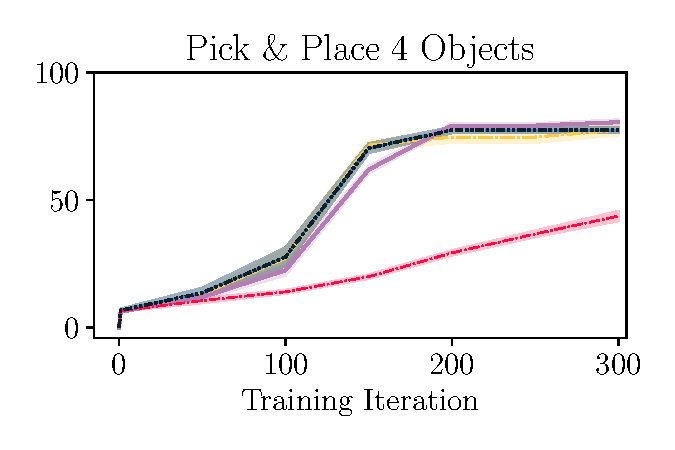
\includegraphics[width=\linewidth]{figures/fpp_construction/construction_pp4_success_monotonous.pdf}
        %\caption{Pick \& Place 4}
    \end{subfigure}
    \begin{subfigure}{.32\linewidth}
        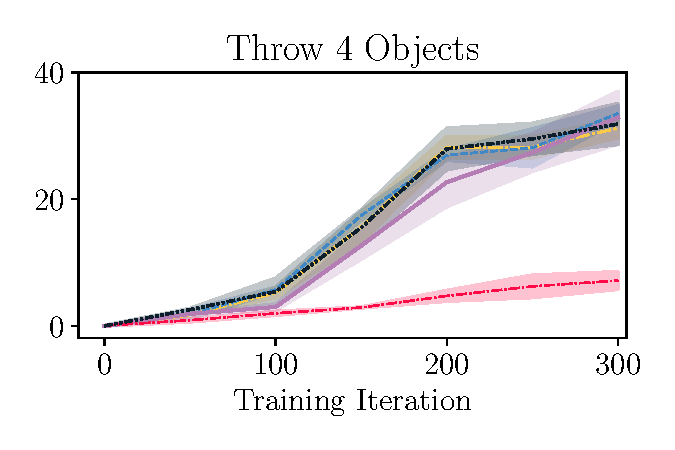
\includegraphics[width=\linewidth]{figures/fpp_construction/construction_throw4_success_monotonous.pdf}
        %\caption{Throw 4}
    \end{subfigure}
    \begin{subfigure}{.32\linewidth}
        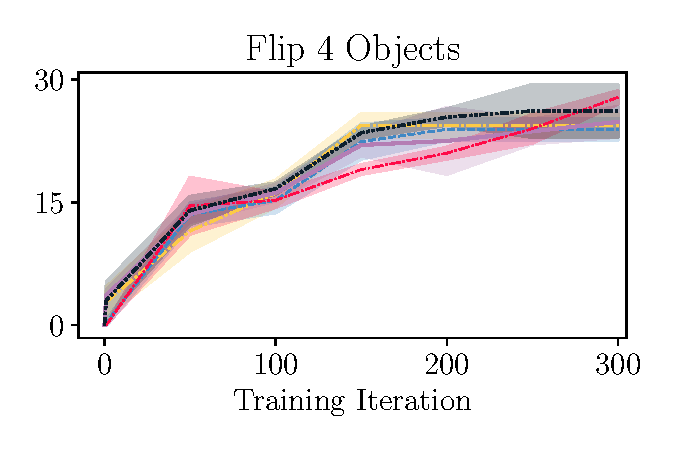
\includegraphics[width=\linewidth]{figures/fpp_construction/construction_flip4_success_monotonous.pdf}
        %\caption{Flip 4}
    \end{subfigure}\\
    
\includegraphics[width=.8\linewidth]{figures/fpp_construction/legend_updated.pdf}
    \caption{\looseness-1 Success rates for pick \& place, throwing and flipping tasks with four objects in the Fetch Pick \& Place Construction environment for \opacex and baselines. \capt{We evaluate task performance via planning zero-shot with models learned using different exploration strategies. We report performance on three independent seeds. \opacex is on par with the best-performing baselines in all tasks.}}
    \label{fig:construction:success_rates}
%\vspace{-0.5cm}
\end{figure}